\documentclass[
	fecha={5 de agosto de 2025},
	palabrasclave={RetoSecundaria, ago2025, álgebra, dif1},
	codigo=minted
]{RetoMatematico}

\usepackage{RetoExtra} % Comandos y paquetes adicionales

\begin{document}
\maketitle
\thispagestyle{empty}

\ejercicio{Esto es un ejemplo de un enunciado propuesto. Cabe la posibilidad de que el enunciado tenga varios apartados:
	\begin{enumerate}[label={\textit{\alph*}}\hspace{0.5pt})]
		\item Apartado 1º (puede ir referenciado).\label{it:1}
		\item Apartado 2º (puede ir referenciado).\label{it:2}
	\end{enumerate}
}{Propuesto por Menganito Flautas.}

Respecto al enunciado, en caso de que el texto debiera ir acompañado de alguna figura/imagen (situada a la derecha del mismo), se recomienda utilizar el siguiente código:
\begin{codigo}{LaTeX}
\begin{cajaejercicio}
	\begin{wrapfigure}{r}{50mm}
        \centering
		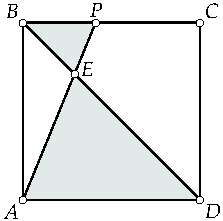
\includegraphics[scale=1]{imagenes/ejemplo-pstricks.pdf}
	\end{wrapfigure}
    \textbf{Ejercicio:} Este es el enunciado ...
\end{cajaejercicio}

\noindent{\sf\color{verdeodi}Propuesto por Menganito Flautas.}
\end{codigo}


\forma

\lipsum[1-2]

\begin{wrapfigure}{r}{37mm}
	\vspace{-4.5mm}
	\centering
	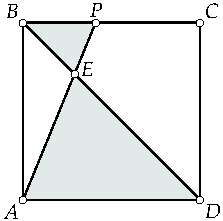
\includegraphics[scale=1]{imagenes/ejemplo-pstricks.pdf}
	\caption{}\label{fig:jmsm1}	
\end{wrapfigure}
Vamos a considerar resolver el problema mediante geometría analítica y optimización de la función <<suma de áreas de los triángulos sombreados>>.

En referencia al apartado \ref{it:1}, si consideramos un sistema de ejes cartesianos centrados en el punto \(A\), y se tiene en cuenta para nuestros cálculos que el cuadrado representado en la figura del enunciado propuesto es de lado unidad (posteriormente se aplicará un factor de escala), se tienen las rectas \(BD\) y \(AP\) que se cortan en el punto \(E\), cuyas coordenadas se obtendrán de resolver el sistema de ecuaciones de dichas rectas. Consideramos por lo tanto que el punto \(P=(a,1)\) (véase la figura \ref{fig:jmsm1}). El sistema a resolver será:
\[
\begin{dcases}
	x+y=1,\\ y=\frac{x}{a}\,,\quad 0\leq a\leq 1.
\end{dcases}
\]
Entonces
\[
x+\frac{x}{a}=1\implies x=\frac{a}{a+1}\implies y=\frac{1}{a+1}\implies E=\left(\frac{a}{a+1}\,,\frac{1}{a+1}\right).
\]

Consideramos a continuación la función \(f(a)\) <<suma de las áreas de los triángulos \(EPB\) y \(EAB\)>>. Entonces
\[
f(a)=A_{\triangle EAB}+A_{\triangle EPB}=\frac{1}{2}\cdot 1\cdot \frac{1}{a+1}+\frac{1}{2}\cdot a\cdot\left(-\frac{1}{a+1}\right)=\frac{a^2+1}{2(a+1)}\,.
\]

Optimizamos la función \(f(a)\):
\[
f'(a)=\frac{2a\big(2(a+1)\big)-2(a^2+1)}{4(a+1)^2}=\frac{a^2+2a-1}{2(a+1)^2}\,,
\]
entonces
\[
f'(a)=0\iff a^2+2a-1=0\implies a=\frac{-2\pm\sqrt{4+4}}{2}\implies\begin{cases}a=-1-\sqrt{2}\Rightarrow\text{No vale},\\a=\sqrt{2}-1.\end{cases}
\]

Puede comprobarse que dicho extremo relativo de la función \(f\big(\sqrt{2}-1\big)\) es un mínimo:
\[
f''(a)=\frac{3a^2+6a+7}{4(a+1)^4}\implies f''\big(\sqrt{2}-1\big)>0\implies f(a)_{\text{mín}}\iff a=\sqrt{2}-1.
\]

Luego \(AB+BP=1+\sqrt{2}-1=\sqrt{2}\). Pero no hemos aplicado el factor de escala al que hacíamos referencia al principio de nuestra resolución, resultando
\[
A_{\square ABCD}=72\ \text{m}^2\implies AB=BC=\sqrt{72}=6\sqrt{2}\ \text{m}.
\]

\enfasis{AB+BP=\sqrt{2}\cdot 6\sqrt{2}=12\ \text{m}}

\ref{it:1} La fórmula propuesta en el enunciado es la conocida como \emph{identidad de Candido} y se puede comprobar desarrollando cada miembro por separado y viendo que coinciden. En efecto, se tiene que
\begin{align*}
	\Bigl(x^2&+y^2+\l(x+y\r)^2\Bigr)^2 = \l(x^2 + y^2\r)^2 + (x+y)^4 + 2\l(x^2 + y^2\r)(x+y)^2\\
	&= \underbrace{x^4 + y^4 + 2x^2y^2}+\underbrace{x^4 + 4x^3y + 6x^2y^2 + 4xy^3 + y^4} + 2\l(x^2 + y^2\r)(x+y)^2\\
	&= 2x^4 + 2y^4 + 8x^2y^2 + 4x^3y + 4xy^3 + 2\l(x^4 + x^2y^2 + 2x^3 y + x^2 y^2 + y^4 + 2xy^3\r)\\
	&= 2\l(2x^4 + 2y^4 + 6x^2y^2 + 4x^3 y + 4xy^3\r)\\
	&= 2\bigl(x^4 + y^4 + \underbrace{x^4 + 4x^3 y + 6x^2y^2 + 4xy^3 + y^4}\bigr)\\
	&= 2\l(x^4 + y^4 + (x+y)^4\r). \tag*{\qedsymbol}
\end{align*}

\ref{it:2} Aplicando la identidad anterior con $x = 23$ e $y = 87$, todo se reduce a calcular los
cuadrados de 23, 87 y de $23 + 87 = 110$ y echar unas sencillas cuentas que pueden hacerse
a mano: \begin{align*}
	\sqrt{\frac{23^4+87^4+110^4}{2}} &= \sqrt{\frac{2\cdot\l(23^4+87^4+110^4\r)}{4}} = \frac{\sqrt{\l(23^2+87^2+110^2\r)^2}}{2}\\
	&= \frac{529 + 7\ 569 + 12\ 100}{2} = \frac{20\ 198}{2} = \num{10099}.
\end{align*} Por lo tanto \enfasis{\sqrt{\frac{23^4+87^4+110^4}{2}} = \num{10099}}


\forma
\ref{it:1} Este resultado puede demostrarse fácilmente expandiendo ambas expresiones y verificando que son idénticas: 
\begin{align*}
    \left(x^2 + y^2 + (x+y)^2\right)^2 &= \left(2x^2 + 2y^2 + 2xy\right)^2 = 4x^4 + 4y^4 + 12x^2y^2 + 8x^3y + 8xy^3\\
    &= 2\left(x^4 + y^4 + \big(x^4 + 4x^3 y + 6x^2y^2 + 4 xy^3 + y^4\big)\right)\\
	&= 2\left(x^4 + y^4 + (x+y)^4\right).
\end{align*}

\ref{it:2} Y el segundo apartado no es sino un corolario de lo anterior: \begin{align*}
    \sqrt{\frac{23^4 + 87^4 + 110^4}{2}} &= \sqrt{\frac{2\left(23^4 + 87^4 + (23+87)^4\right)}{4}} \overset{\ref{it:1}}{=} \sqrt{\frac{\left(23^2 + 87^2 + 110^2\right)^2}{4}}\\
	&= \frac{23^2 + 87^2 + 110^2}{2} = \frac{(2\cdot 11 + 1)^2 + (2\cdot 43 + 1)^2 + (2\cdot 55)^2}{2}\\
	&= 2\left(11^2 + 43^2 + 55^2\right) + 109.
\end{align*} Haciendo estos últimos cómputos a mano (no son sino productos de números relativamente pequeños) se llega a \num{10099} como resultado final.

\forma

El ejercicio puede ser resuelto de numerosas maneras alternativas distintas.

\nseccion{Método por ordenador} %Sección numerada
Con el siguiente código de \mathematica, digo Python, podemos comprobar que en efecto es cierto para $x,y\leq \num{10000}$, y como ese número es muy grande, el teorema ha de ser cierto por narices:
\begin{codigo}{python}
def main() -> None:
	for x in range(1, 10_001):
		for y in range(1, 10_001):
			assert (x**2 + y**2 + (x+y)**2)**2\
			    == 2*(x**4 + y**4 + (x+y)**4)

if __name__ == '__main__': main()
\end{codigo}

\nseccion{Texto de ejemplo} %Sección numerada
Aquí va un poco de <<lorem ipsum>> para que los resolutores no se queden solos en esta nueva página.

\lipsum[1]

\begin{wrapfigure}{r}{40mm}
	\vspace{-5mm}
	\centering
	
\includegraphics[width=42mm]{imagenes/autor}
	\caption{}
\end{wrapfigure}
\lipsum[2-3]

A continuación, ponemos una referencia bibliográfica \cite[véase][p. 25]{beato1944}. Otra forma de poner la referencia es \citet[p. 25]{beato1944}, o bien, \citeauthor{beato1944}, \citeyear[p. 25]{beato1944}.



\resolutores{\hypersetup{urlcolor=verdeodi}\href{mailto:fulanitodemaracaibo@gmail.com}{Fulanito de Maracaibo} y \href{mailto:xyz@gmail.com}{el proponente}.}

\begin{thebibliography}{A}
	
	\bibitem[Pérez-Beato Olivier(1944)]{beato1944} \textsc{Pérez-Beato Olivier}, Manuel. (1944). \textit{Manual-Formulario de Geometría Analítica}, S.A.E.T.A.
	
\end{thebibliography}

\end{document}
